\begin{frame}{Context : KoroiBot project}
\begin{center}
  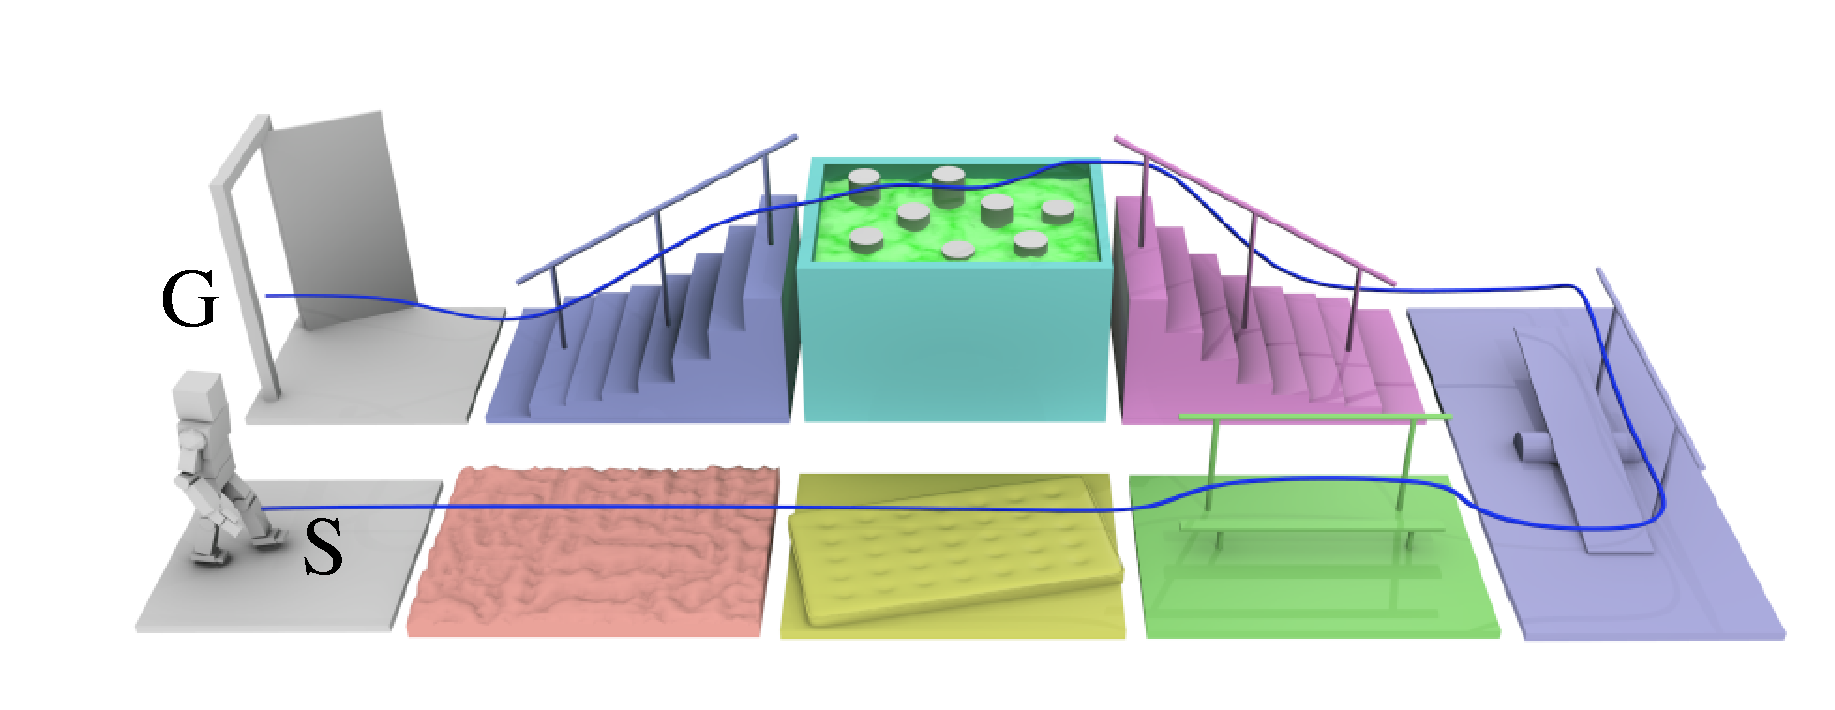
\includegraphics[width=\linewidth]{koroibot/KoroibotChallengeEnhanced.pdf}
  \begin{tikzpicture}[remember picture, overlay]
%    \draw[help lines] (0,0) grid (-1,1);
%    \node at (0,0) {(0,0)};
    \draw[line width=1.5pt, color=red](-10,1) ellipse (0.8cm and .6cm);
    \draw[line width=1.5pt, color=red](-8,1) ellipse (1.1cm and .6cm);
    \draw[line width=1.5pt, color=red](-3.3,1) ellipse (1.1cm and .6cm);
    \draw[line width=1.5pt, color=red](-3.5,3) ellipse (1.0cm and .8cm);
    \draw[line width=1.5pt, color=red](-7.7,3) ellipse (1.0cm and .8cm);
    \draw[line width=1.5pt, color=red](-5.7,3) circle (1.0cm);
  \end{tikzpicture}
\end{center}
%\begin{itemize}
%  \item 
%\end{itemize}

Goal : enhance the ability of humanoid robots to walk in a dynamic and versatile way, and to bring them closer to human capabilities.
\end{frame}


\begin{frame}{Project Partners}
\vspace*{-0.7cm}
\begin{columns}
\column{0.6\linewidth}
\begin{center}
  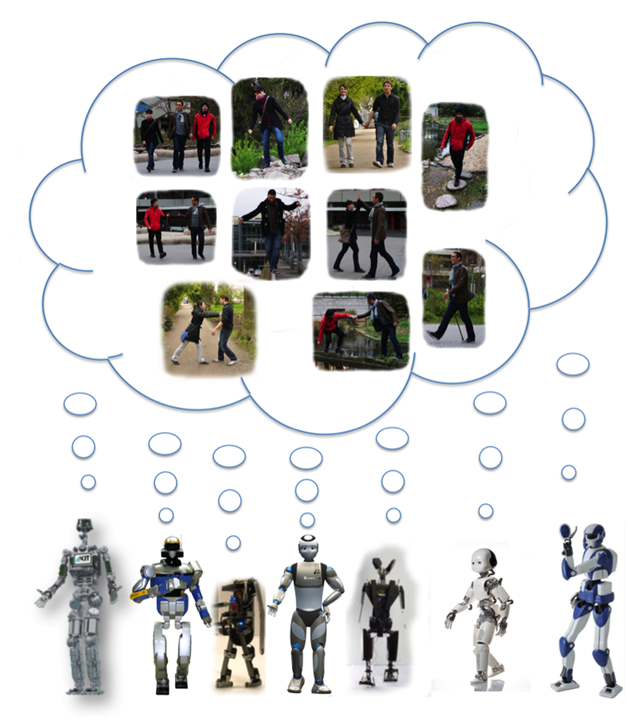
\includegraphics[height=0.75\textheight]{koroibot/situations_v2.png}
\end{center}
\vspace*{-0.5cm}
  \small{ \hspace*{0.3cm} ARMAR-IV \hspace*{0.4cm}  Leo \hspace*{0.4cm} TUlip \hspace*{0.6cm} HRP-4 }\\
  \small{ \hspace*{1.7cm} \textcolor{blue!50!black}{\textbf{HRP-2}} \hspace*{0.1cm} \textcolor{blue!50!black}{\textbf{Romeo}} \hspace*{0.3cm} iCube}
\column{0.4\linewidth}
\begin{center}
  
\includegraphics[height=0.1\textheight]{koroibot/logos/cnrs.png}\\
  
\includegraphics[height=0.1\textheight]{koroibot/logos/iit.png}\\
  
\includegraphics[height=0.1\textheight]{koroibot/logos/tud.png}\\
  
\includegraphics[height=0.1\textheight]{koroibot/logos/hd.png}\\
  
\includegraphics[height=0.1\textheight]{koroibot/logos/kit.png}\\
  
\includegraphics[height=0.1\textheight]{koroibot/logos/ut.png}\\
  
\includegraphics[height=0.1\textheight]{koroibot/logos/wi.png}
\end{center}

\end{columns}
%\begin{itemize}
%  \item 
%\end{itemize}
\end{frame}

%\fullFrameImage{figures/koroibot/components2.png}{}

%
%\begin{frame}{Context}
%\begin{center}
%   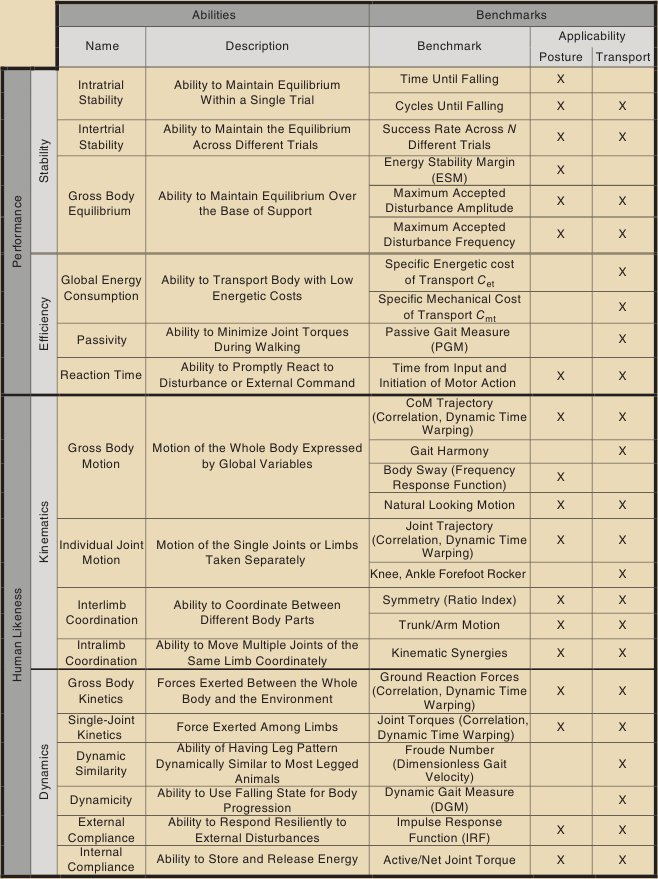
\includegraphics[width=0.90\linewidth]{koroibot/KPIabilities.jpg}
%\begin{tikzpicture}[remember picture, overlay]
%    %\draw[help lines, color=blue] (-8,0) grid (8,25);
%    %\node [color=red] at (0,0) {\textbf (0,0)};
%    %\node [color=red] at (0,20) {\textbf (0,20)};
%    %\node [color=red] at (0,10) {\textbf (0,10)};
%    \draw[line width=1.5pt, color=red](-4.6,16.2) ellipse (2.2cm and .43cm);
%    \draw[line width=1.5pt, color=red](-4.6,13.3) ellipse (2.2cm and .43cm);
%    \draw[line width=1.5pt, color=red](-4.6,12.45) ellipse (2.2cm and .43cm);
%  \end{tikzpicture}
%\end{center}
%%\begin{itemize}
%%  \item 
%%\end{itemize}
%\end{frame}
%
%
%
%\begin{frame}{Context}
%\begin{center}
%   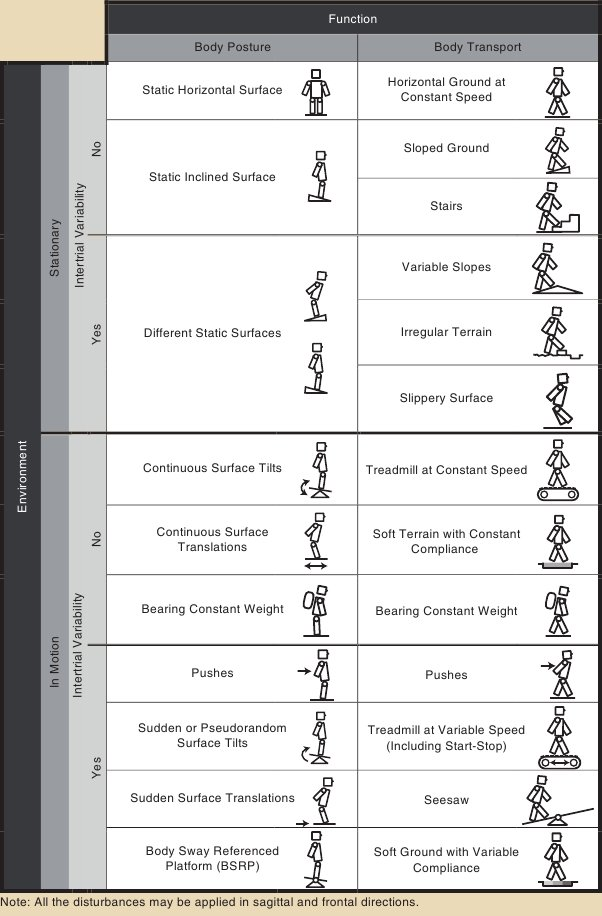
\includegraphics[height=0.9\textheight]{koroibot/KPIexperiment.jpg}
%\begin{tikzpicture}[remember picture, overlay]
%    %\draw[help lines, color=blue] (-8,0) grid (8,25);
%    %\node [color=red] at (0,0) {\textbf (0,0)};
%    %\node [color=red] at (0,20) {\textbf (0,20)};
%    %\node [color=red] at (0,10) {\textbf (0,10)};
%    \draw[line width=1.5pt, color=red](-3.9,19.7) ellipse (2cm and .5cm);
%    \draw[line width=1.5pt, color=red](-3.9,16.9) ellipse (2cm and .5cm);
%    \draw[line width=1.5pt, color=red](-3.9,9.0) ellipse (2cm and .5cm);
%    \draw[line width=1.5pt, color=red](-9.5,7.25) ellipse (2cm and .5cm);
%  \end{tikzpicture}
%\end{center}
%%\begin{itemize}
%%  \item 
%%\end{itemize}
%\end{frame}

\begin{frame}{Problem presentation}

\begin{columns}


%Continuous formulation :
%
%\begin{align*}
%\text{min}  &\quad f({\bm q},{\bm v},t) \\
%\text{s.t.} &\quad
%g({\bm q},{\bm v},t) < 0 \nonumber \\
%&\quad h({\bm q},{\bm v},t) = 0 \nonumber
%\end{align*}

%\vspace*{2.5cm}

\column{0.45\linewidth}

Optimal Control Formulation :

\begin{align*}
\hspace{-3em}	\underset{\substack{\hspace{0.2em} \underline{\bm x}, \; \underline{\bm u}} }{\min } \ \ \  
	& & \hspace{-3em} {\sum_{s=1}^S} \int_{t_{s}}^{t_{s}+\Delta t_s\hspace{-4em}} \ell_{s} (\bm x, \bm u) \, dt \\
	s.t. & \forall t & \dot{\bm{x}} = \text{dyn}(\bm x, \bm u) \\
	&  \forall t& \bm\phi \in \mathcal{K} \\
  &  \forall t& {\bm x} \in \mathcal{B}_x \\ 
  &  \forall t& {\bm u} \in \mathcal{B}_u \\ 
	& & \bm x(0) = \bm x_{0} \\
	& & \bm x(T) \in \mathcal{X}_*
\end{align*}

\column{0.5\linewidth}

\vspace*{0.7cm}
\begin{itemize}
\item $x$ : state (pose,velocity,..)
\item $u$ : control (forces)
\item $\bm\phi$ : forces applied to the system
\item $\text{dyn}$ : dynamics of the system
\item $\mathcal{K}$ : balance criteria
\item $\mathcal{B}_x$ \& $\mathcal{B}_u$ : Bounds on $x$ \& $u$\\[0.5cm]
\item Initial condition
\item Final condition (task)
\end{itemize}

\end{columns}

\end{frame}


\begin{frame}{Dynamics}
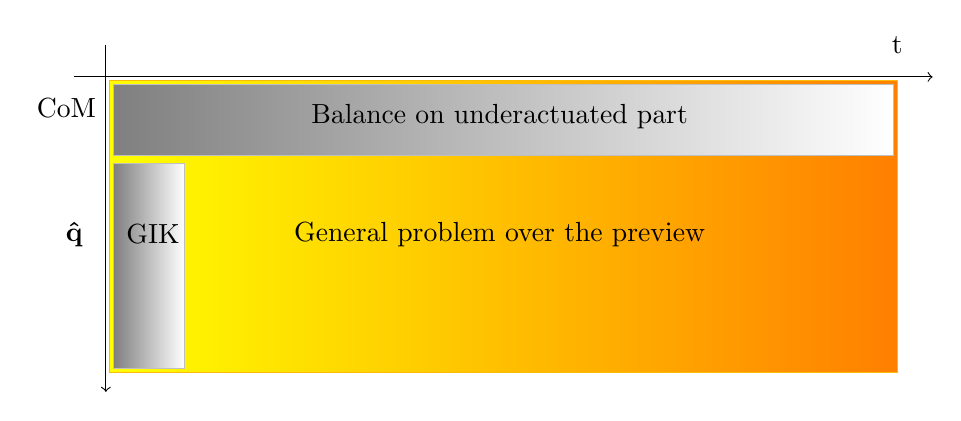
\begin{tikzpicture}
  \draw [->] (-0.4,0) -- (10.5,0);
  \draw [->] (0,0.4) -- (0,-4);
  \shadedraw[left color=yellow, right color= orange, draw=yellow!50!orange](0.05,-0.05) rectangle (10.05,-3.75);
  \shadedraw[left color=gray, right color= white, draw=gray!50!white] (0.1,-0.1) rectangle (10,-1.0);
  \shadedraw[left color=gray, right color= white, draw=gray!50!white](0.1,-1.1) rectangle (1,-3.7);
  \draw (10.05,0.4) node {t};
  \draw (-0.5,-0.4) node {CoM};
  \draw (-0.4,-2.0) node {${\bf \hat{q} }$};
  \draw (5,-0.5) node {Balance on underactuated part};
  \draw (0.6,-2.0) node {GIK};
  \draw (5,-2.0) node {General problem over the preview};
\end{tikzpicture}
\end{frame}

\begin{frame}{State Of Art}

\begin{center}
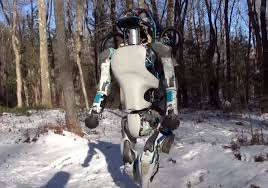
\includegraphics[trim={0.0cm 0.0cm 3.0cm 0.0cm}, clip,
height=0.4\textheight ,keepaspectratio]
{figures/stateoftheart/bostondynamics.jpeg}\hspace*{0.3cm}
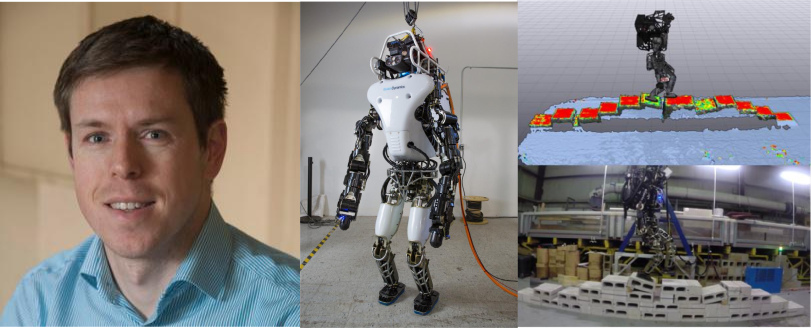
\includegraphics[trim={20.0cm 0.0cm 0.0cm 0.0cm}, clip,
height=0.4\textheight , keepaspectratio]
{figures/stateoftheart/humanoids2015.png}\hspace*{0.3cm}
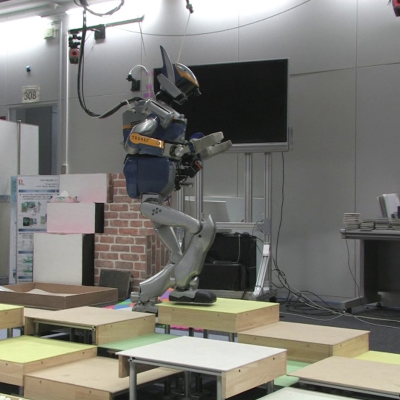
\includegraphics[height=0.4\textheight , keepaspectratio]
{figures/stateoftheart/rsj30_humanoid_navigaion_nishiwaki_aist.png}

[Boston Dynamics 2016] %\hspace*{0.5cm}
[Fallon Humanoids 2015] %\hspace*{0.5cm}
[Nishiwaki IJRR 2012]
%trim={<left> <lower> <right> <upper>}
\end{center}

\end{frame}

\begin{frame}{State Of Art}
\vspace*{-0.7cm}
\begin{small}

\begin{minipage}{0.4\textwidth}
\begin{minipage}{0.4\textwidth}
Linearized Inverted Pendulum Model :
\begin{itemize}
\item $\dot{\bf \am} = 0$
\item $\ddot{c}^z = 0$
\item $c^z = cst$
\end{itemize}
\end{minipage}
\begin{minipage}{0.2\textwidth}
\begin{align*}
& cop^x = {c}^x - \frac{c^z}{g}\ddot{c}^x \\
& cop^y = {c}^y - \frac{c^z}{g}\ddot{c}^y \\
& cop^z = 0
\end{align*}
\end{minipage}
\end{minipage}
%
\begin{minipage}{0.4\textwidth}
\begin{align*}
&m (\ddot{\mbf{c}}-\mbf{g}) = \sum\limits_{k=1}^{K} \; {^0}R_k \mbf{f}_k
\\
&m \mbf{c} \times (\ddot{\mbf{c}}-\mbf{g}) + \dot{\bf \am} = \sum\limits_{k=1}^{K} \mbf{p}_k \times {^0}R_k \mbf{f}_k  + \bm{\tau}_k
\end{align*}
\end{minipage}\\
%
\begin{minipage}{0.4\textwidth}
\begin{align*}
m (\ddot{\mbf{c}}-\mbf{g}) = \sum\limits_{k=1}^{K} \; {^0}R_k \mbf{f}_k
\\
m \mbf{c} \times (\ddot{\mbf{c}}-\mbf{g}) + \dot{\bf \am} = \sum\limits_{k=1}^{K} \mbf{p}_k \times {^0}R_k \mbf{f}_k  + \bm{\tau}_k
\end{align*}
\end{minipage}
%
\begin{minipage}{0.4\textwidth}
\begin{minipage}{0.4\textwidth}
Linearized Inverted Pendulum Model :
\begin{itemize}
\item $\dot{\bf \am} = 0$
\item $\ddot{c}^z = 0$
\item $c^z = cst$
\end{itemize}
\end{minipage}
\begin{minipage}{0.2\textwidth}
\begin{align*}
& cop^x = {c}^x - \frac{c^z}{g}\ddot{c}^x \\
& cop^y = {c}^y - \frac{c^z}{g}\ddot{c}^y \\
& cop^z = 0
\end{align*}
\end{minipage}
\end{minipage}

\end{small}


\begin{tikzpicture}[remember picture, overlay]
%  \draw[help lines] (0,0) grid (-1,1);
%  \node at (0,0) {(0,0)};
  \draw [line width=1.5pt, color=txtcolor2] (5.3,0.0) rectangle (11.7,2.7);
\end{tikzpicture}

\end{frame}